\subsubsection{Cluster-coefficient}
$c_N$ characterizes the connectivity of a node. It's given by the number of edges between neighbors of a node divided by the maximum number of edges among them. An undirected (directed) Graph with $k$ nodes may have $\frac{k(k-1)}{2}$ ($(k-1)k$) edges, since each node can be connected with $(k-1)$ neighbors.\\
\begin{itemize}[label={}]
\item Undirected: $c_N=\frac{e}{k(k-1)/2}=\frac{2e}{k(k-1)}$ where $e=\#$ edges between neighbors
\item Directed: $c_N=\frac{e}{k(k-1)}$
\end{itemize}
$c_N$ obviously takes values between $0$ and $1$, where $1$ corresponds to a fully connected graph or clique.\\
The graphs clustering coefficient is simply given by the mean of all nodes $c_\mathcal{G}=\frac{1}{m}\sum\limits_{N=1}^m c_N$ where $m=\#$ nodes of $\mathcal{G}$\\
Remark: In real biological networks $C_\mathcal{G}$ is typically low. There exists only a relatively small number of hubs, i.e. nodes that are highly connected to dense clusters.\\
\begin{figure}[H]
	\begin{center}
		\begin{multicols}{2}
			\begin{figure}[H]
				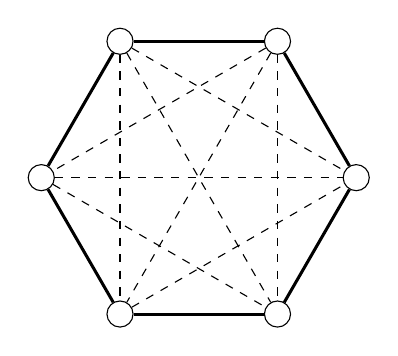
\begin{tikzpicture}
					\foreach \x in {1,...,6}{
						\node[draw,shape=circle,name=A\x] at ({60*\x}:2){};
					}
					\foreach \x in {1,...,5}{
						\foreach \y in {\x,...,6}{
							\draw[dashed] (A\x)--(A\y);
						};
					};
					\foreach \x \y in {1/2,2/3,3/4,4/5,5/6,6/1}{
						\draw[line width=1.1 pt] (A\x)--(A\y);
					};
				\end{tikzpicture}
			\end{figure}
			\begin{figure}[H]
				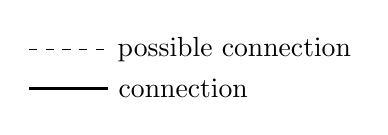
\begin{tikzpicture}
					\draw[dashed] (0,0)--(1,0)node[right]{possible connection};
					\draw[line width=1.1 pt] (0,-0.5)--(1,-0.5)node[right]{connection};
				\end{tikzpicture}
			\end{figure}\columnbreak
			\begin{figure}[H]
				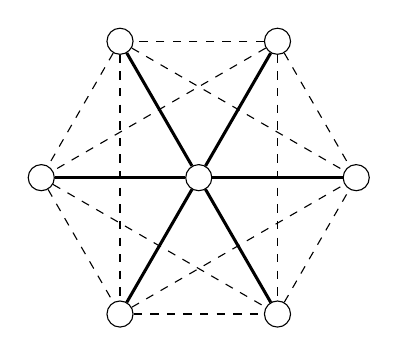
\begin{tikzpicture}
					\foreach \x in {1,...,6}{
						\node[draw,shape=circle,name=A\x] at ({60*\x}:2){};
					}
					\foreach \x in {1,...,5}{
						\foreach \y in {\x,...,6}{
							\draw[dashed] (A\x)--(A\y);
						};
					};
					\node[draw,fill=white,shape=circle,name=A7] at (0:0){};
					\foreach \x in {1,...,6}{
						\draw[line width=1.1 pt] (A\x)--(A7);
					};
				\end{tikzpicture}
			\end{figure}
			\begin{figure}[H]
				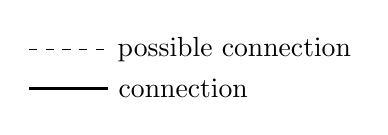
\begin{tikzpicture}
					\draw[dashed] (0,0)--(1,0)node[right]{possible connection};
					\draw[line width=1.1 pt] (0,-0.5)--(1,-0.5)node[right]{connection};
				\end{tikzpicture}
			\end{figure}
		\end{multicols}
	\end{center}
\end{figure}
\begin{figure}[H]
\begin{multicols}{2}
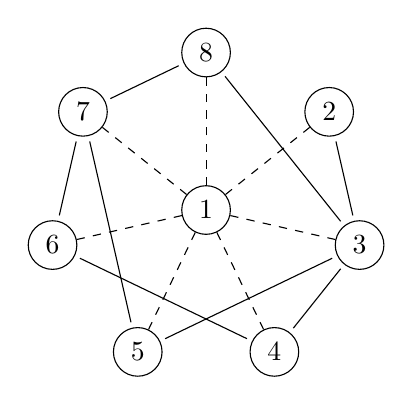
\begin{tikzpicture}
\node[draw,shape=circle,name=a1] at (0,0){$1$};
\foreach \x in {2,...,8}{
	\node[draw,shape=circle,name=a\x] at ({360/7*(1-\x)+90}:2){$\x$};
	\draw[dashed] (a1)--(a\x);
};
\foreach \x \y in {2/3,3/4,3/5,3/8,7/5,7/8,7/6,4/6}{
	\draw[shorten <= 2pt, shorten >= 2pt] (a\x)--(a\y);
};
\end{tikzpicture}\\\columnbreak
\begin{itemize}[label={$\bullet$}]
\item undirected graph
\item 7 neighbours of 1
\item 8 edges connecting neighbours
\item $c_1=\frac{8}{7\cdot\frac{6}{2}}=\frac{8}{21}$
\item $c_5=2\cdot\left(3\cdot\frac{2}{2}\right)^{-1}=\frac{2}{3}$
\end{itemize}
\end{multicols}
\end{figure}
\noindent Another important characteristic of a graph $\mathcal{G}$ with $m$ nodes is its degree distributio
\begin{equation*}
P(k)=\frac{m_k}{m}\text{, where $m_k=\#$ nodes with degree $k$}
\end{equation*}
$P(k)$ is obviously normalized.
\begin{itemize}[label={}]
\item \underline{Random graphs}: $P(k)$= Binomial distribution
\item \underline{Biological graphs}: $P(k)\propto k^{-\gamma}$ (scale-free network)\\
Scale-free networks are dominated by a few hubs and many sparsely connected nodes
\begin{itemize}[label={$-$}]
\item The shortest paths, i.e. the shortest distance between randomly selected nodes is significantly lower than for random graphs, where it is $\sim\log(m)$ ($m=\#$ nodes)\\
\grqq{}Small-world\grqq{} networks\footnote{Barabasi Rev. Mod. Phys} are scale-free networks with high clustering coefficients. Typically average path-lengths are $\num{2}-\num{5}$ steps.
\end{itemize}
\end{itemize}
\subsubsection{Construction of small world networks}
\begin{itemize}[label={$-$}]
\item The edges of new node are connected to an existing node with a probability $\sim\text{deg}(N) \to \gamma =3$
\item Variations of the mechanism lead to other values of $\gamma$
\end{itemize}
\subsubsection{Dependencies among network components}
\begin{itemize}[label={$-$}]
\item \underline{Causality analysis}: True cause must be neccessary and sufficient to execute an effect (Galileo).\\
Causes in networks are often studied with statistical methods, from which one obtains typically cause-effect diagrams which are directed graphs. In biology, networks often contain cycles, which complicate the analysis.
\item \underline{Mutual information}: The mutual dependence of two variables is often much easier to acces. Typical question: How likely is it that gene $X$ is expressed if gene $Y$ is expressed as well?
\end{itemize}
%\clearpage
\subsubsection{Bayesian construction (cond. probabilities)}
We first recall some elementary results of probability theory
\paragraph{Random variables} A random variable $X$ is a quantity which may take different values with vertain probabilities.
\paragraph{Entropy $H(x)$} The entropy measures the uncertainty associated with the variable x. The uncertainty may depend on the knowledge of another random variable (e.g. two genes, that are likely to be expressed together)
\subparagraph{Joint entropy $H_I(X,Y)$} = uncertainty in finding $X$ and $Y$.
\subparagraph{Conditional Entropy $H(X|Y)$} = uncertainty for $X$ given $Y$.
\begin{equation*}
\leadsto H_I(X,Y)=H(X)+H(Y|X)=H(Y)+H(X|Y)
\end{equation*}
mutual information: $I(X,Y)=\left[H(X)+H(Y)\right]-H_I(X,Y)$
